%TC:group tabular 1 1
\section{Function calls}

\begin{figure}[H]
  \centering
  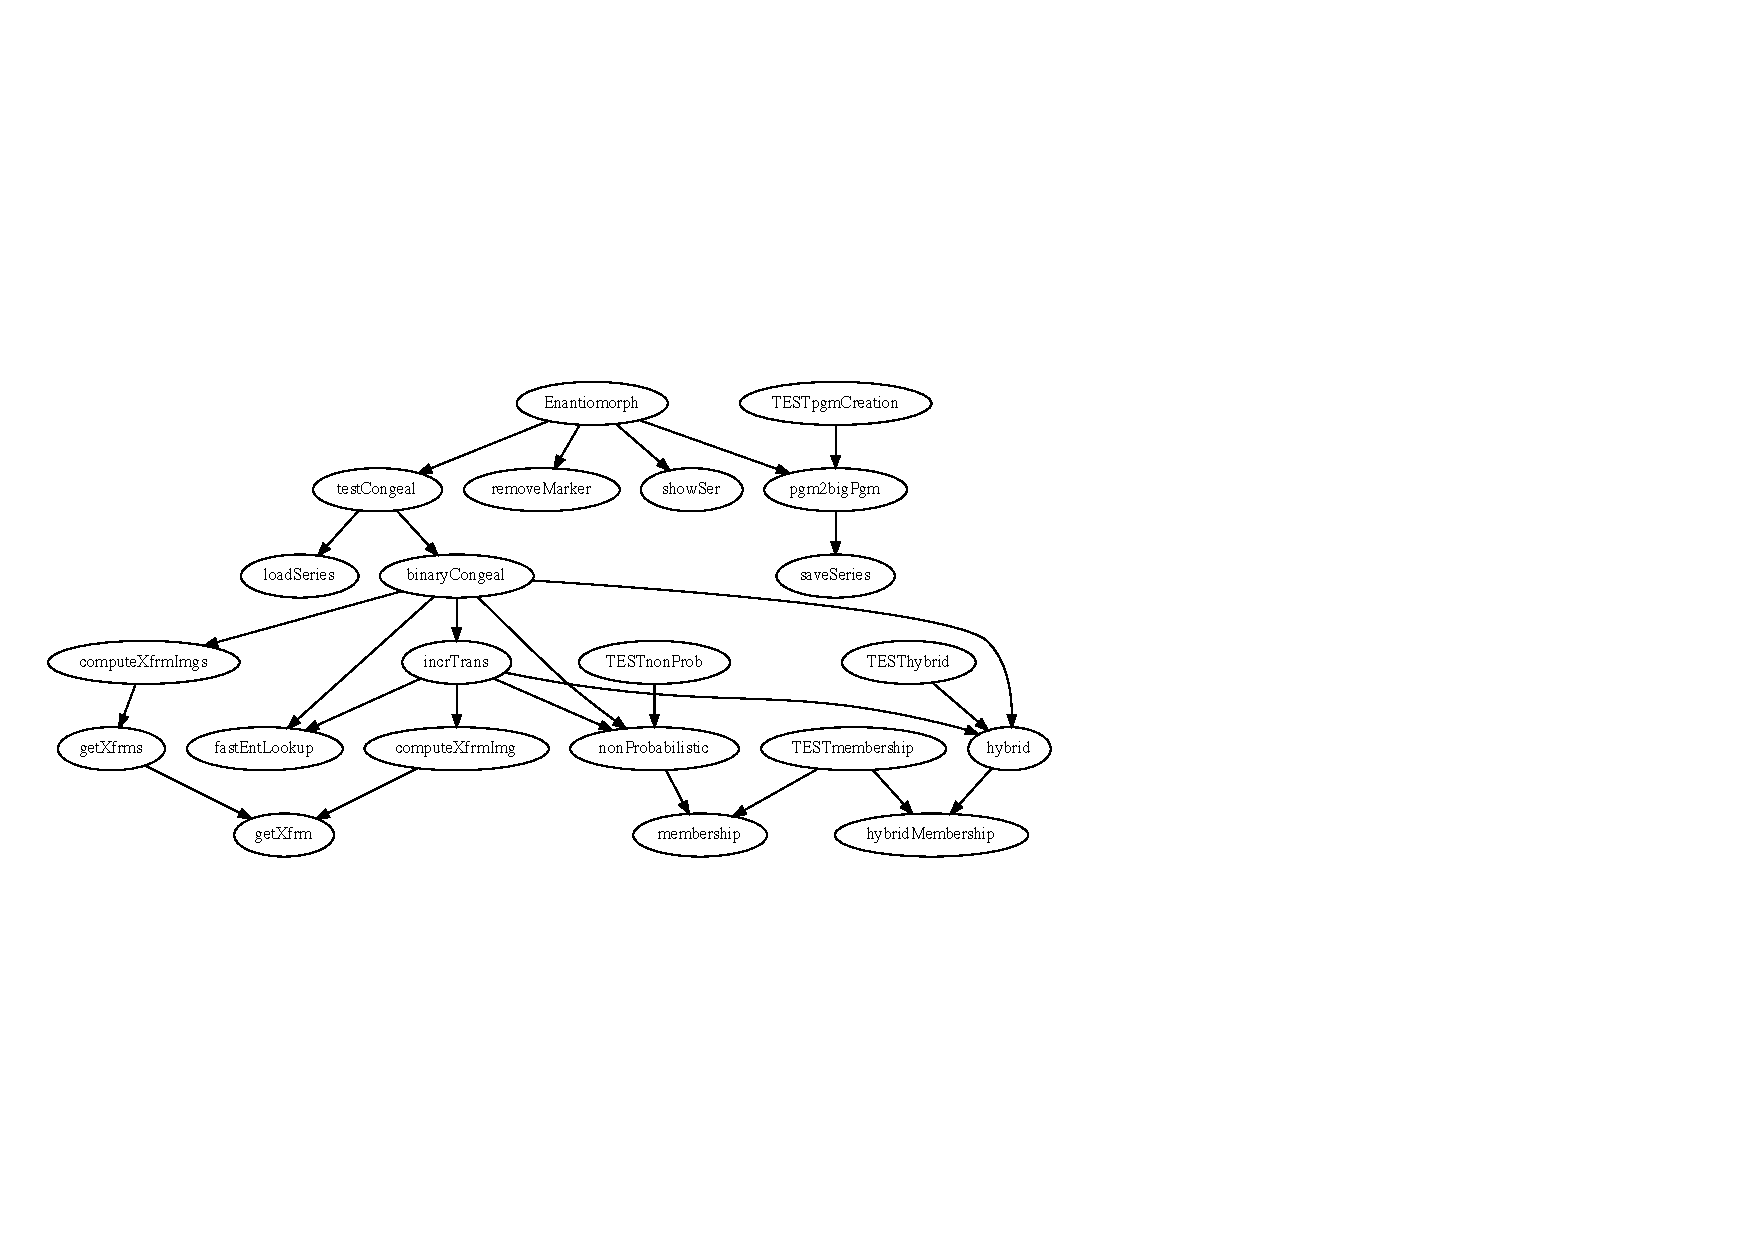
\includegraphics[width=\textwidth,clip,trim=0mm 50mm 110mm 50mm]{Chapter2/software-img/function_call_1.pdf}
  \caption{Function calls through the application.}
  \label{fig:data-flow}
\end{figure}

Figure \ref{fig:data-flow} shows which function/script calls which through the application, all the way up to \texttt{Enantiomorph}, the \acrshort{GUI}. This diagram shows the integration of new, modified and existing functions/scripts in the code-base, as listed in Appendix \ref{appendix:code}.

Initial diagrams like this were helpful especially at the beginning of the project, due to working with an existing code-base. It was advantageous to see which functions were directly being called, and where the new functions for fuzzy entropy and membership would fit in. However Figure \ref{fig:data-flow} is representative of the final design and was generated once development had been completed.

\newpage
\section{Vectorisation}
\label{sec:vectorisation}

Vectorisation is the process to replace loop-based code with MATLAB matrix and vector operations. As stated in the MATLAB documentation \cite{vectorisation}, Vectorisation is important for several reasons:

\begin{enumerate}
    \item Appearance - more concise, more like what is seen in textbooks
    \item Less error prone - less for loops = less lines of code for errors to appear
    \item Performance - vectorised code usually runs a lot faster
\end{enumerate}

Whilst appearance as an advantage in the MATLAB documentation, it's concise nature often makes it harder for developers to read - as will be briefly discussed in Subsection \ref{ssec:trans}.

The initial implementations of both \texttt{membership.m} and \texttt{nonProbabilistic.m} contained for loops, so experimentation was run before, during and after vectorisation to evaluate the supposed performance increase.

\begin{figure}[H]
  %\iffalse
  \centering
    \begin{tikzpicture}
      \begin{axis}[
          width = 11cm,
          ybar,
          bar width=4pt,
          ylabel={Time (secs)},
          xlabel={Iterations},
          xtick={1,...,5},
          nodes near coords,
          every node near coord/.append style={font=\scriptsize,
                xshift=-6pt,  yshift=+5pt,anchor=west},
          nodes near coords align={vertical},
          legend pos=outer north east,
          legend style={cells={align=left}},
          ]
        \addplot table[x=Iteration, y=Pre optimisation, col sep=comma] {Chapter2/technical-img/time.csv};
        \addlegendentry{Pre-optimisation \\ (for loops) \\};
        \addplot table[x=Iteration, y=Partial optimisation, col sep=comma] {Chapter2/technical-img/time.csv};
        \addlegendentry{Partial optimisation \\ (just membership.m) \\};
        \addplot table[x=Iteration, y=Full optimisation, col sep=comma] {Chapter2/technical-img/time.csv};
        \addlegendentry{Full optimisation \\ (both membership.m \& \\ nonProbabilistic.m) \\};
      \end{axis}
    \end{tikzpicture}
    \caption{Time per iteration before, during and after vectorisation}
    \label{fig:time-per-iteration}
    %\fi
\end{figure}

Figure \ref{fig:time-per-iteration} demonstrates the time taken per iteration, in the same environment, to run the \texttt{binaryCongeal.m} \footnote{The function which calls the specified entropy algorithm.} function. A marked improvement can be seen just by vectorising the \texttt{membership.m} function, and further improvements once the \texttt{nonProbabilistic.m} function for Non-Probabilistic entropy was vectorised.

%http://pgfplots.sourceforge.net/gallery.html
\begin{figure}[H]
  %\iffalse
  \begin{center}
    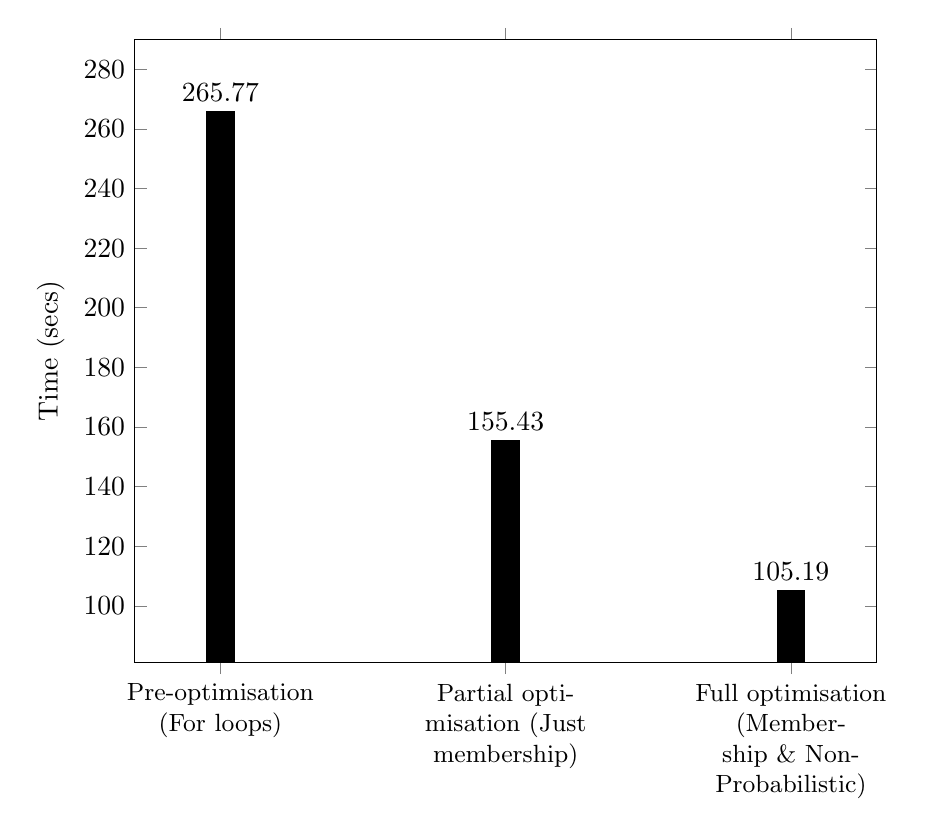
\begin{tikzpicture}
      \begin{axis}[
        width= 11cm,
        symbolic x coords={Pre-optimisation (For loops),Partial optimisation (Just membership),Full optimisation (Membership \& Non-Probabilistic)},
        x tick label style={font=\small,text width=2.5cm,align=center},
        ybar,
        enlargelimits=0.15,
        legend style={at={(0.5,-0.2)},
          anchor=north,legend columns=-1},
        ylabel={Time (secs)},
        xtick={Pre-optimisation (For loops),Partial optimisation (Just membership),Full optimisation (Membership \& Non-Probabilistic)},
        nodes near coords,
    	  nodes near coords align={vertical},
        ]
        \addplot[ybar,fill] coordinates {
    (Pre-optimisation (For loops),265.771186)
    (Partial optimisation (Just membership),155.432352)
    (Full optimisation (Membership \& Non-Probabilistic),105.188263) };
      \end{axis}
    \end{tikzpicture}
    \caption{A comparison of the total time to run five iterations prior to vectorisation, during (part vectorisation) and post-vectorisation.}
    \label{fig:total-time}
  \end{center}
  %\fi
\end{figure}

Figure \ref{fig:total-time} outlines the total time taken to run five iterations of Non-Probabilistic Entropy before vectorisation, once vectorisation was complete on the \texttt{membership.m} function, and finally after full vectorisation.

\newpage
\section{Testing}

Prior to the project beginning, it was outlined that this project would follow a \acrfull{TDD} practice. In \acrshort{TDD}, the developer first writes a test, which will fail due to the lack of corresponding functionality. They would then go on to implement the functionality desired by the test. Finally, any refactoring of the initial test and/or code would take place.

However due to the nature of the project, it became increasingly more difficult to follow given the research which had to be undertaken alongside development. This led to a change from \acrshort{TDD} to Retrospective Testing, all tests would be written post-functional-implementation. This is a more traditional approach to testing, and still catches the same errors which might occur during \acrshort{TDD}.

\subsection{Unit Tests}

Unit Tests were completed using MATLAB's Unit Testing Framework \cite{testing}, which covers all the ways in which you can program in MATLAB:

\begin{itemize}
  \item Script-Based Unit Tests
  \item Function-Based Unit Tests
  \item Class-Based Unit Tests
  \end{itemize}

The majority of my work in MATLAB was function-based, so this was the style followed for unit tests. As Figure \ref{fig:unit-test-results} demonstrates, all Unit tests passed.

\begin{figure}[H]
  \centering
  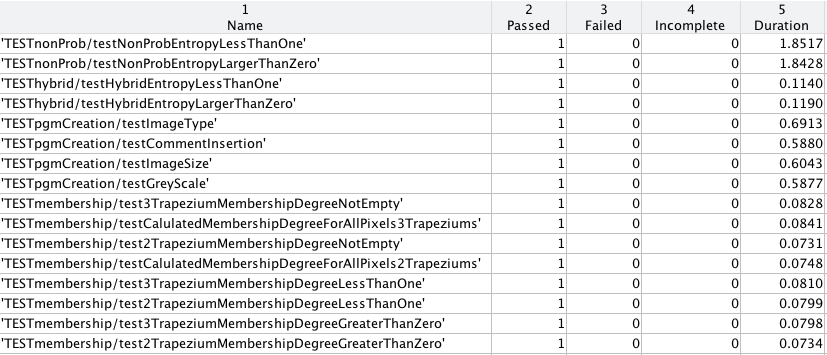
\includegraphics[width=\textwidth]{Chapter2/software-img/test-results.png}
  \caption{Results from MATLAB Unit Tests.}
  \label{fig:unit-test-results}
\end{figure}

\newpage
\subsection{Acceptance Tests}

Acceptance tests are when each `requirement' is assessed in turn to assure its completion. In this project, as there was no firm requirements at the beginning of the process, the User Stories which were derived over the project duration will be assessed against. In \acrfull{XP}, a user story is not considered to be complete until the time in which it passes its acceptance test, as stating on the \acrshort{XP} website \cite{Acceptance_Tests}.

Table \ref{table:acceptance} outlines the results from the Acceptance Tests run. The left-most column \say{User Story Reference} aligns with Table \ref{table:User Stories}, where more detail on each story can be found.

\begin{center}
  \small
  \begin{longtable}{| p{2cm} | p{6cm} | p{2cm}  | p{1.5cm} |}
    \hline
      \textbf{User Story Reference} & \textbf{Expected Outcome} & \textbf{Actual \newline Outcome} & \textbf{Pass/Fail} \\ \hline \endhead
      1 & Image is loaded into the system & As expected & Pass \\ \hline
      2 & Membership array is passed out of the membership function and is usable in other functions & As expected & Pass \\ \hline
      3 & Images are aligned using Non-Probabilistic entropy and the output \& entropy outputs are realistic & As expected & Pass \\ \hline
      4 & Images are aligned using the metric the user has selected when running the function & As expected & Pass \\ \hline
      6 & The number of iterations is run as specified by the User, then function stops & As expected & Pass \\ \hline
      8 & Images are aligned using Shannon entropy and the output \& entropy outputs are realistic & As expected & Pass \\ \hline
      9 & Image(s) selected to be loaded into the GUI is displayed & As expected & Pass \\ \hline
      12 & Image box where input image appears goes blank after Clear button is selected & As expected & Pass \\ \hline
      13 & Images are aligned using Hybrid entropy and the output \& entropy outputs are realistic & As expected & Pass \\ \hline
      14 & Images are aligned using the chosen alignment metric & As expected & Pass \\ \hline
      15 & The number of iterations is run as specified by the User, then function stops & As expected & Pass \\ \hline
      16 & When an input image is loaded in, Metadata is displayed in the GUI about the image & As expected & Pass \\ \hline
      17 & After \Gls{Congealing}, the user can press the \say{See all Mean images} button and a new Figure displays the mean image after each iteration & As expected & Pass \\ \hline
      18 & After \Gls{Congealing}, the user can press the \say{See Adjusted Inputs} button and a new Figure displays the adjusted input images after the final iteration  & As expected & Pass \\ \hline
      21 & Image box where output image appears goes blank after Clear button is selected along with all other fields & As expected & Pass \\ \hline
      22 & Image is displayed larger in a new Figure & As expected & Pass \\ \hline
      23 & Save file dialog appears with a sensible name suggested (i.e. final image - alignment-chosen - number of iterations) & As expected & Pass \\ \hline
      24 & When \say{Entropy details} button is selected, a new Figure appears with a graph showing entropy decrease. Final Entropy \& time taken also displays in the main GUI & As expected & Pass \\ \hline
      25 & Egg-timer appears when \Gls{Congealing} Algorithm is running & As expected & Pass \\ \hline
      \caption{Acceptance Test results}
      \label{table:acceptance}
  \end{longtable}
\end{center}
